% ============================================================
% Baseball2Vector — CVPR Workshop (CVsports) style draft
% ------------------------------------------------------------
% HOW TO USE ON OVERLEAF:
%  1) Start from the official CVPR template project
%     (search "CVPR 2026" in Overleaf templates), which provides
%     cvpr.sty and the review/final options.
%  2) Replace the main .tex with this file.
%  3) Copy the three figures from outputs/figures/ into a
%     figures/ folder in the Overleaf project:
%       - fig1_zscore_area_vs_war.png
%       - matched_profile_distances.png
%       - roi_coefficients.png
%  Numbers in this draft are verified against data/processed/
%  v3_results.csv, outputs/tables/, and the versioned artifacts in
%  academic_validation_experiments/results/ and tables/.
% ============================================================

\documentclass[10pt,twocolumn,letterpaper]{article}

% --- CVPR template package (from the official template project) ---
\usepackage[pagenumbers]{cvpr}   % use [review] for the review version

\usepackage{graphicx}
\usepackage{amsmath,amssymb}
\usepackage{booktabs}
\usepackage{multirow}
\usepackage{xurl}
\usepackage[pagebackref,breaklinks,colorlinks]{hyperref}

\def\paperID{****}
\def\confName{CVPR Workshop (CVsports)}
\def\confYear{2026}

\begin{document}

%%%%%%%%% TITLE
\title{Baseball2Vector: An Interpretable Five-Dimensional Skill Representation of MLB Position Players}

\author{Jaeseok Choi\\
I2SLAB, Sungkyunkwan University\\
{\tt\small jaeseok.choi@skku.edu}
}

\maketitle

%%%%%%%%% ABSTRACT
\begin{abstract}
Modern baseball evaluates players through raw measurements, sabermetric composites, and the traditional 20--80 scouting scale, yet scalar summaries compress qualitatively different profiles onto one axis. We propose \emph{Baseball2Vector}, a five-dimensional season-level representation of Power, Contact, Plate Discipline, Defense, and Speed. These adapted dimensions are reported on a bounded 20--80-formatted relative scale and are not professional scout grades. Using FanGraphs statistics for 2{,}309 MLB hitter-seasons (2021--2025, $\geq$100 PA), we compare Z-score averaging, per-dimension PCA, and an exploratory joint variational autoencoder. Z-score area has the strongest descriptive alignment with WAR ($r=0.81$), although shared inputs make this an internal-consistency check rather than independent validation. In a leakage-controlled next-season evaluation, Ridge regression using only the 2024 vector predicts 2025 wRC+ with MAE 18.02, $R^2=0.280$, and Spearman $\rho=0.508$ over 358 returning players; adding age and PA gives $R^2=0.289$ but no statistically clear incremental gain. Both models outperform league-mean and carry-forward baselines, while a raw-statistic baseline could not be reconstructed from the archived processed data. Year-to-year stability is lower for low-PA observations and for Defense and Speed. Moreover, scalar-matched different players have larger standardized profile distances than same-player adjacent seasons (median 1.001 vs.\ 0.714), supporting the representation's ability to retain profile differences hidden by aggregate value. Concurrent dimension-change regressions and synthetic perturbations remain descriptive associations and sensitivity analyses, not forecasts or causal development estimates.
\end{abstract}

%%%%%%%%% BODY
\section{Introduction}
\label{sec:intro}

Evaluating and comparing player ability is central to modern baseball. For front offices, accurately gauging a player's ability underpins the decisions that matter most: which prospects to draft or sign, and which players to deploy in which roles. For players themselves, an objective account of where their strengths and weaknesses lie is a prerequisite for targeted development. And for fans, much of the enjoyment of the sport comes from understanding \emph{how} a player is good---which tools carry them---and from counterfactual imagination: ``what if this player added power?'' In all three cases, what is needed is not merely a ranking but a \emph{representation}: a compact, interpretable description of a player that supports comparison, communication, and reasoning.

Existing answers are only partial. Sabermetric composites such as WAR and wRC+ condense a player's contribution into a single number, which is invaluable for ranking but discards profile information: a slugger with poor contact skills and a well-rounded defender with modest power can receive similar scores while being entirely different players. Conversely, raw tracking statistics preserve detail but can overwhelm interpretation. The traditional 20--80 scouting scale sits between these extremes and provides a widely shared vocabulary in the sport, but it is typically assigned through expert observation and projection rather than derived reproducibly from public season statistics \cite{mcdaniel2014}.

We propose \emph{Baseball2Vector}, which represents each position-player season as a five-dimensional vector across Power, Contact, Plate Discipline, Defense, and Speed, computed from public statistics and displayed on a bounded 20--80-formatted relative scale. This is an adapted skill taxonomy rather than a reconstruction of the canonical five scouting tools. The vector can be visualized as a pentagon; its area is analyzed as an exploratory geometric summary, while the vector itself retains the dimension-level profile that the area discards.

Our contributions are as follows:
\begin{itemize}
  \item We formalize a mapping from public season statistics to a five-dimensional, 20--80-formatted relative profile and compare Z-score averaging, per-dimension PCA, and an exploratory joint variational autoencoder.
  \item We distinguish descriptive alignment from prediction: Z-score area has the strongest shared-input alignment with WAR, while a season-$t$ Ridge model is evaluated prospectively against league-mean and carry-forward baselines on 2024$\to$2025.
  \item We quantify year-to-year stability by dimension and PA stratum and show that scalar-matched players retain substantially different skill profiles.
  \item We treat dimension-delta regression as a contemporaneous transition association and synthetic perturbations as model-sensitivity diagnostics, not forecasts, causal effects, or development prescriptions.
\end{itemize}

\section{Related Work}
\label{sec:related}

\paragraph{Measurement-level statistics.}
Baseball Savant\footnote{\url{https://baseballsavant.mlb.com}} publicly releases a large volume of in-game physical measurements (exit velocity, sprint speed, arm strength, and so on) captured by the Statcast system. These measurements are enormously useful to teams, players, and fans, but they are \emph{measured outcomes}: interpreting them requires at least one further stage of aggregation and normalization before they speak to player ability.

\paragraph{Sabermetric value composites.}
FanGraphs\footnote{\url{https://www.fangraphs.com}} and Baseball Reference\footnote{\url{https://www.baseball-reference.com}} publish composite value metrics such as WAR and wRC+ that summarize a player's total contribution. These have become the lingua franca of player valuation, but they carry known limitations: different publishers use different formulas, so the ``same'' metric takes different values across sources; and by construction a single scalar cannot distinguish players who reach the same value through different skill profiles.

\paragraph{The 20--80 scouting scale.}
Long before Statcast, scouts graded players on a 20--80 scale centered at 50, with each 10-point step conventionally corresponding to approximately one standard deviation. The canonical position-player tools are Hit, Power, Run, Field, and Throw; plate discipline is commonly treated as a component of the Hit tool rather than a separate sixth tool \cite{mcdaniel2014}. The scale preserves profile information that value composites discard, but grades are traditionally assigned through expert observation and projection. Baseball2Vector borrows the visual range, not the full semantics or validity of professional scouting grades.

\paragraph{Baseball player representations.}
Prior work has learned latent representations of baseball players from plate-appearance interactions. Alcorn's \emph{batter2vec/pitcher2vec} predicts at-bat outcomes from neural player embeddings \cite{alcorn2016}, while Heaton and Mitra learn time-varying 72-dimensional player-form representations from sequences of Statcast events \cite{heaton2021}. These approaches emphasize predictive or contextual embeddings. Our narrower goal is an explicitly named, season-level profile whose dimensions can be inspected directly; accordingly, interpretability is prioritized over embedding capacity.

\paragraph{Vector representations in NLP.}
In natural language processing, Word2Vec demonstrated that words can be embedded in a semantic vector space in which geometric proximity reflects semantic similarity and, famously, arithmetic on vectors captures analogical relations (\emph{king} $-$ \emph{man} $+$ \emph{woman} $\approx$ \emph{queen}) \cite{mikolov2013}. This result established distributed vector representations as a general tool for turning discrete entities into computable objects.

\paragraph{This work.}
Inspired by these threads, Baseball2Vector uses public season-level statistics to encode observed player performance as a low-dimensional, interpretable vector. Unlike black-box player embeddings, each dimension is assigned a baseball-relevant name; unlike scalar composites, the representation preserves profile structure. Synthetic modifications of a vector are used only to probe the fitted model's sensitivity, not to claim that an intervention on one skill would cause the predicted change in value.

\section{Methodology}
\label{sec:method}

\subsection{Tool Selection}
The canonical five tools for position players are Hit, Power, Run, Field, and Throw \cite{mcdaniel2014}. Public FanGraphs season statistics do not provide a satisfactory, consistently available measure of throwing-arm ability for hitters across the entire study window. We therefore define an \emph{adapted five-dimensional taxonomy}: \textbf{Power}, \textbf{Contact}, \textbf{Plate Discipline}, \textbf{Defense}, and \textbf{Speed}. This taxonomy omits the traditional Throw tool and separates plate discipline from the broader Hit tool. We consequently refer to these quantities as \emph{dimensions} rather than canonical scouting tools, and do not interpret them as direct substitutes for professional present or future grades.

\subsection{Data Collection and Preprocessing}
\label{sec:data}
We collect season-level statistics from FanGraphs (via the \texttt{pybaseball} library\footnote{\url{https://github.com/jldbc/pybaseball}}) for all MLB hitters with at least 100 plate appearances in each of the 2021--2025 seasons, yielding 2{,}309 player-season rows. Cross-sectional analyses retain all rows. For longitudinal analyses, display names are conservatively linked to stable FanGraphs/MLBAM identifiers through the Chadwick Register \cite{chadwickRegister}. This procedure uniquely matches 2{,}286 rows from 818 players; 23 ambiguous or unmatched rows are excluded rather than resolved from performance context. In particular, the two distinct Max Muncy rows in 2025 are both excluded from longitudinal analysis because the archived processed file lacks source identifiers. Constituent statistics are grouped by dimension as follows:
\begin{itemize}
  \item \textbf{Contact}: Contact\%, K\%, AVG, xBA, SwStr\%
  \item \textbf{Power}: ISO, SLG, HardHit\%, Barrel\%, maxEV, EV, HR/FB
  \item \textbf{Speed}: Spd, BsR, UBR, wSB
  \item \textbf{Plate Discipline}: BB\%, O-Swing\%, Swing\%, BB/K
  \item \textbf{Defense}: Def, Fld
\end{itemize}
Statistics for which lower is better (K\%, SwStr\%, O-Swing\%, Swing\%) are sign-flipped before aggregation so that higher always means better.

FanGraphs defines \emph{Def} as fielding runs plus positional adjustment \cite{fangraphsDef}. Consequently, averaging standardized Def and Fld repeats the fielding component, mixes fielding with positional value, and retains playing-time dependence. We preserve the published construction for reproducibility but treat Defense as the least cleanly identified dimension.

Because rate statistics computed over few plate appearances are noisy, we apply empirical-Bayes-style shrinkage before scoring: each rate statistic is pulled toward its season league average using a pre-specified prior strength expressed in PA equivalents (e.g., 60 PA for K\%, 120 PA for BB\%, and 500 PA for AVG). These are heuristic hyperparameters motivated by published stabilization-point summaries \cite{fangraphsSampleSize}, rather than estimated population priors. Statistics that are already composite measures (e.g., Spd and Def) are left untouched. All standardization is computed \emph{within season} to respect era and run-environment differences. The archived processed file contains only final dimension scores, not the pre-shrinkage constituent statistics; therefore literal no-shrinkage and stronger-shrinkage reconstructions were not possible in the present audit, and we make no robustness claim for these hyperparameters.

\subsection{Encoding Schemes}
Each dimension $t$ has a set of constituent statistics $S_t$. We compare three ways of collapsing $S_t$ into a single dimension score.

\paragraph{Z-score averaging.}
Each statistic in $S_t$ is standardized to zero mean and unit variance over the per-season player population; the dimension score is the mean of these Z-scores. Because several inputs within and across dimensions are correlated or algebraically related (e.g., AVG and SLG, or K\% and BB/K), the resulting averages are transparent composites rather than estimates of independent latent abilities.

\paragraph{PCA.}
The statistics in each $S_t$ co-vary as facets of a related performance construct (e.g., ISO, SLG, and Barrel\% all reflect power). We apply PCA within each dimension group and take the first principal component as the dimension score, capturing its dominant shared axis of variation.

\paragraph{JointVAE.}
Per-dimension encoders cannot capture cross-dimension structure. We therefore also train a single variational autoencoder over all constituent statistics jointly \cite{kingma2014}: a shared MLP encoder maps the full statistic set to a 5-dimensional latent with a full posterior covariance parameterized through its Cholesky factor ($\Sigma = LL^{\top}$), and five group-specific decoders reconstruct the input groups. Latent dimensions are assigned post hoc to named dimensions using correlations with anchor statistics (e.g., ISO for Power), with signs flipped where needed. This procedure does not guarantee disentanglement or unique semantic identification; accordingly, the JointVAE is treated as an exploratory representation baseline. Posterior off-diagonal covariance describes dependence in the approximate latent posterior and is not interpreted directly as a causal or population-level tool trade-off. Results are reported for a fixed seed; stability across random seeds remains to be assessed.

\paragraph{20--80 scaling.}
Whatever the encoder, dimension scores are mapped to a bounded 20--80-formatted range by an affine min--max transformation over the pooled 2021--2025 population, so that the observed extremes anchor 20 and 80. The result is a vector $\mathbf{v} = (v_{\text{Con}}, v_{\text{Pow}}, v_{\text{Spd}}, v_{\text{Def}}, v_{\text{Dis}}) \in [20,80]^5$. This transformation is not the classical scouting convention of mean 50 and approximately 10 points per standard deviation. It is cohort-dependent: adding a new extreme observation can change every player's grade. We therefore describe the outputs as \emph{20--80-formatted relative scores}, not scouting grades.

\subsection{Pentagon Area as a Geometric Summary}
For visualization, $\mathbf{v}$ is drawn as a radar chart: five axes at equal $72^\circ$ intervals. We analyze the area of the resulting pentagon as a compact geometric descriptor, computed by decomposing it into five triangles:
\begin{equation}
A(\mathbf{v}) = \tfrac{1}{2}\sin\!\left(\tfrac{2\pi}{5}\right) \sum_{i=1}^{5} v_i\, v_{i+1},
\label{eq:area}
\end{equation}
with indices cyclic. Because Eq.~\ref{eq:area} is a sum over adjacent pairs, the area depends on the ordering of axes. We quantify this sensitivity in Sec.~\ref{sec:results}. Area is therefore not proposed as an invariant overall-value metric; it is a lossy visualization-derived summary whose behavior helps motivate retaining the full vector.

\subsection{Alignment Protocol}
As an internal-consistency check, we compute Pearson correlations between pentagon area and three established metrics---WAR, wRC+, and OPS---over all 2{,}309 season-rows, separately for each encoding scheme. These are pooled, descriptive correlations. Several constituent statistics also contribute directly or indirectly to the comparison metrics; moreover, repeated seasons from the same player are not independent observations. The analysis therefore does not establish external construct validity or predictive performance.

\subsection{Dimension-Delta Regression and Model Sensitivity}
\label{sec:roi-method}
To study how concurrent changes in the representation relate to changes in established metrics, we construct 1{,}414 consecutive-season transitions from 567 stably identified players, with features $\Delta\mathbf{v} \in \mathbb{R}^5$ and targets $\Delta$wRC+, $\Delta$WAR, and $\Delta$OPS. We fit (i) a linear regression on the five deltas and (ii) a random forest on the five starting levels and five deltas. We compare shuffled five-fold cross-validation, player-grouped five-fold cross-validation, and a temporally held-out association check trained on transitions ending by 2023 ($n=701$) and tested on 2024$\to$2025 ($n=358$). Even the last split is not a forecast: every predictor $\Delta\mathbf{v}$ contains season-$t+1$ information. We probe local fitted-model sensitivity by applying a synthetic $+5$-grade perturbation to one dimension at a time. This is neither a causal intervention nor an estimate of return on investment.

\subsection{Prospective and Robustness Validation}
\label{sec:validation-method}
For a genuine next-season test, predictors contain only information observed through season $t$. We train on 1{,}056 returning-player transitions ending in 2022--2024 and reserve all 358 matched 2024$\to$2025 transitions as a fixed test set. The primary target is 2025 wRC+; a rate-normalized secondary target is WAR per 600 PA (WAR600). We compare a training-set league-mean baseline, previous-season carry-forward, Ridge regression using only the five season-$t$ dimensions, and Ridge using the vector plus age and PA. Ridge regularization is selected using player-grouped folds inside the training period; imputation and scaling are fitted on training data only. A raw-statistic baseline was planned but cannot be reconstructed because the archived processed file does not contain the constituent statistics. We report MAE, $R^2$, and Spearman $\rho$, with 95\% intervals from 2{,}000 player-level bootstrap resamples of the fixed test set.

We assess temporal reliability separately from prediction. For each adjacent-season pair, we compute dimension-wise Pearson correlations and a standardized Euclidean distance after standardizing each dimension over the pooled cohort. Correlations use 2{,}000 player-cluster bootstrap resamples and are stratified by the lower PA of the two seasons. Finally, we ask whether the vector distinguishes profiles hidden by scalar value. Same-player adjacent-season distances are compared with distances between different players in the same season matched closely on wRC+ and WAR and, as a reference, PA-stratified random same-season pairs. Because matching reuses observations, intervals describe this constructed comparison rather than an independent population experiment.

\section{Results}
\label{sec:results}

\subsection{Quantitative Alignment}
Table~\ref{tab:corr} reports Pearson correlations between pentagon area and established value metrics for the three encodings, and Fig.~\ref{fig:scatter} shows the corresponding scatter for the Z-score encoding against WAR.

\begin{table}[t]
\centering
\caption{Pearson correlation between pentagon area and established value metrics, by encoding scheme (2021--2025, $n=2{,}309$ season-rows). Brackets are 95\% confidence intervals from a player-level cluster bootstrap (2{,}000 resamples; players, not season-rows, are the resampling unit, since a player's several seasons are not independent draws). A paired bootstrap on the same resamples confirms Z-score's advantage over PCA, though only 0.01--0.02 in magnitude, is statistically significant (95\% CI on the difference excludes 0) for all three metrics; the larger gap to JointVAE (0.05--0.16) is significant a fortiori.}
\label{tab:corr}
\small
\begin{tabular}{lccc}
\toprule
Encoding & WAR & wRC+ & OPS \\
\midrule
Z-score averaging & \textbf{0.81} {\scriptsize[0.78, 0.83]} & \textbf{0.65} {\scriptsize[0.61, 0.68]} & \textbf{0.63} {\scriptsize[0.59, 0.66]} \\
PCA               & 0.79 {\scriptsize[0.77, 0.82]} & 0.63 {\scriptsize[0.60, 0.67]} & 0.61 {\scriptsize[0.57, 0.65]} \\
JointVAE          & 0.74 {\scriptsize[0.71, 0.77]} & 0.51 {\scriptsize[0.47, 0.55]} & 0.49 {\scriptsize[0.44, 0.53]} \\
\bottomrule
\end{tabular}
\end{table}

\begin{figure*}[t]
\centering
\includegraphics[width=0.75\linewidth]{figures/fig1_zscore_area_vs_war.png}
\caption{Pentagon area (Z-score encoding) vs.\ WAR over all 2{,}309 season-rows ($r=0.81$). The pooled correlation is descriptive and partly reflects statistics shared by the representation and WAR.}
\label{fig:scatter}
\end{figure*}

Four observations follow. First, Z-score averaging has the strongest descriptive alignment with all three metrics, with PCA close behind and the JointVAE lower. This result favors the transparent baseline for the present purpose, but it does not show that learned encodings are generally inferior. Second, although Z-score's and PCA's marginal confidence intervals in Table~\ref{tab:corr} overlap substantially, a paired bootstrap on the same player resamples---which accounts for the fact that all three encodings are computed on the same players and are themselves highly correlated with each other---shows Z-score's edge over PCA is small (0.01--0.02 in $r$) but statistically significant for all three metrics, with a larger, likewise significant gap to JointVAE (0.05--0.16); so the ordering in Table~\ref{tab:corr} is not an artifact of sampling noise, even though eyeballing the marginal intervals alone would suggest otherwise. Third, the observed ceiling near $r \approx 0.8$ versus WAR is consistent with equal weighting across dimensions and with the different construction of WAR; it should not be interpreted as a geometry-independent theoretical limit. Fourth, recomputing area under every axis permutation yields narrow correlation bands for all three encodings ($r$ vs.\ WAR: Z-score $[0.79, 0.82]$, PCA $[0.78, 0.81]$, JointVAE $[0.74, 0.76]$; comparable bands hold for wRC+ and OPS), although individual rankings can remain unstable. Notably, PCA is the most permutation-sensitive of the three encodings, both in absolute terms and as a fraction of its own correlation, so Z-score's advantage over the alternatives should be attributed to its higher, significant correlation with value metrics rather than to any special robustness to the pentagon's axis ordering.

\subsection{Prospective Prediction and Temporal Stability}
\label{sec:prospective-results}
Table~\ref{tab:prospective} reports the fixed 2024$\to$2025 test. The five-dimensional Ridge model improves wRC+ MAE over carry-forward by 4.33 points (95\% paired-bootstrap CI $[2.89,5.87]$), improves $R^2$ by 0.391 $[0.261,0.540]$, and improves rank correlation by 0.073 $[0.011,0.138]$. Adding age and PA changes MAE by only 0.005 $[-0.371,0.370]$ and $R^2$ by 0.009 $[-0.013,0.031]$ relative to the vector-only model; thus these two covariates show no clear incremental benefit in this test. The secondary WAR600 result is directionally consistent: the augmented model obtains MAE 1.553 $[1.420,1.686]$, $R^2=0.223$ $[0.134,0.305]$, and $\rho=0.439$ $[0.350,0.529]$, whereas carry-forward has negative $R^2$ ($-0.140$). These results establish modest next-season signal among players who return with at least 100 PA, not universal player forecasting. A constituent raw-statistic model is unavailable, so the experiment does not establish that compression into five dimensions improves on all source information.

\begin{table*}[t]
\centering
\caption{Prospective 2025 wRC+ prediction for 358 returning players. Models are trained on 1{,}056 earlier transitions. Brackets are 95\% player-level bootstrap intervals on the fixed test set. Spearman correlation is undefined for the constant league-mean predictor.}
\label{tab:prospective}
\small
\begin{tabular}{lccc}
\toprule
Model & MAE $\downarrow$ & $R^2$ $\uparrow$ & Spearman $\rho$ $\uparrow$ \\
\midrule
League mean & 22.27 [20.51, 24.00] & $-0.001$ [$-0.016$, 0.000] & --- \\
Previous-season wRC+ & 22.35 [20.51, 24.39] & $-0.102$ [$-0.298$, 0.078] & 0.449 [0.355, 0.535] \\
B2V Ridge & \textbf{18.02} [16.51, 19.68] & 0.280 [0.179, 0.375] & 0.508 [0.423, 0.588] \\
B2V Ridge + age + PA & \textbf{18.02} [16.52, 19.62] & \textbf{0.289} [0.192, 0.382] & \textbf{0.522} [0.438, 0.600] \\
\bottomrule
\end{tabular}
\end{table*}

Across 1{,}414 stable-ID adjacent-season pairs, player-clustered correlations are highest for Discipline (0.760; 95\% CI $[0.726,0.789]$), Contact (0.734; $[0.697,0.765]$), and Power (0.730; $[0.691,0.761]$), and lower for Speed (0.626; $[0.580,0.668]$) and Defense (0.568; $[0.516,0.614]$). Reliability rises with playing time: for 100--249 PA pairs, correlations range from 0.463 (Defense) to 0.719 (Discipline), whereas for 500+ PA they range from 0.661 to 0.789. This supports interpreting the vectors as noisy season summaries, especially at low PA, rather than fixed latent traits. A median raw cosine similarity of 0.996 is not emphasized because the positive 20--80 offset mechanically inflates it; standardized Euclidean distance is more informative.

\subsection{Qualitative Analysis: Profiles Behind Geometric Summaries}
Table~\ref{tab:top10} lists the top-10 season-rows by pentagon area (Z-score encoding) with their established metrics. Elite seasons by Ronald Acu\~na Jr., Shohei Ohtani, Aaron Judge, Juan Soto, Jose Ramirez, and Bobby Witt Jr.\ appear, but area also ranks profiles whose established offensive values differ substantially. Judge's 2024 vector is $(58, 79, 44, 37, 65)$ in (Contact, Power, Speed, Defense, Discipline) order---extreme Power with elite Discipline---while Soto's 2024 vector $(64, 66, 29, 44, 71)$ is carried by Discipline, and Witt's 2024 vector $(67, 60, 53, 60, 41)$ is more distributed. Ohtani's 2024 season $(59, 74, 72, 37, 48)$ pairs elite Power with elite Speed. These examples illustrate profile readability rather than external validation of the scores.

\begin{table}[t]
\centering
\caption{Top-10 season-rows by pentagon area (Z-score encoding) with established metrics.}
\label{tab:top10}
\scriptsize
\setlength{\tabcolsep}{3pt}
\begin{tabular}{lrrrr}
\toprule
Player (Season) & Area & WAR & wRC+ & OPS \\
\midrule
Ronald Acu\~na Jr.\ (2023) & 8644.6 &  9.2 & 171 & 1.012 \\
Shohei Ohtani (2024)       & 8089.1 &  9.0 & 180 & 1.036 \\
Aaron Judge (2022)         & 7794.7 & 11.1 & 206 & 1.111 \\
Juan Soto (2021)           & 7639.3 &  6.8 & 164 & 0.999 \\
Jose Ramirez (2021)        & 7568.0 &  6.4 & 140 & 0.893 \\
Aaron Judge (2024)         & 7523.9 & 11.3 & 220 & 1.159 \\
Bobby Witt Jr.\ (2024)     & 7349.6 & 10.5 & 169 & 0.977 \\
Nicky Lopez (2021)         & 7155.2 &  5.5 & 104 & 0.744 \\
Juan Soto (2024)           & 7128.0 &  8.3 & 181 & 0.989 \\
Bobby Witt Jr.\ (2025)     & 7102.5 &  8.0 & 130 & 0.852 \\
\bottomrule
\end{tabular}
\end{table}

The list also contains an instructive outlier: Nicky Lopez's 2021 season ranks eighth by area despite a merely league-average bat (104 wRC+, .744 OPS). His vector $(63, 30, 66, 71, 48)$ is the mirror image of a slugger's---elite Defense and Speed with well below-average Power---and the symmetric area rewards that balance. Notably, area here agrees with WAR (5.5, driven by defense and baserunning) far better than with the offense-only metrics, illustrating both what the equal-weight summary captures and what it overweights.

\subsection{Scalar-Matched Profile Diversity}
\label{sec:matched-profile}
Figure~\ref{fig:matched-profile} strengthens the qualitative claim with a pre-specified matching analysis. The median standardized distance is 0.714 for same-player adjacent seasons (95\% bootstrap CI $[0.696,0.726]$), 1.001 for different players closely matched on both wRC+ and WAR ($[0.980,1.028]$), and 1.197 for PA-stratified random same-season pairs ($[1.176,1.228]$). The scalar-matched minus same-player median difference is 0.288 $[0.263,0.319]$. Thus aggregate value matching removes some, but not most, profile heterogeneity. As an illustration selected by a fixed rule---both players at 400+ PA and nearest the 90th percentile of matched-pair distance---Alex Verdugo and Luis Robert Jr.\ in 2024 have nearly identical scalar outcomes (wRC+ 85 vs.\ 84; WAR 0.6 vs.\ 0.6) but a distance of 1.787. Verdugo is higher in Contact and Discipline, while Robert is higher in Power and Speed. The distributional comparison, rather than this single example, is the primary evidence that the vector preserves information hidden by scalar value.

\begin{figure*}[t]
\centering
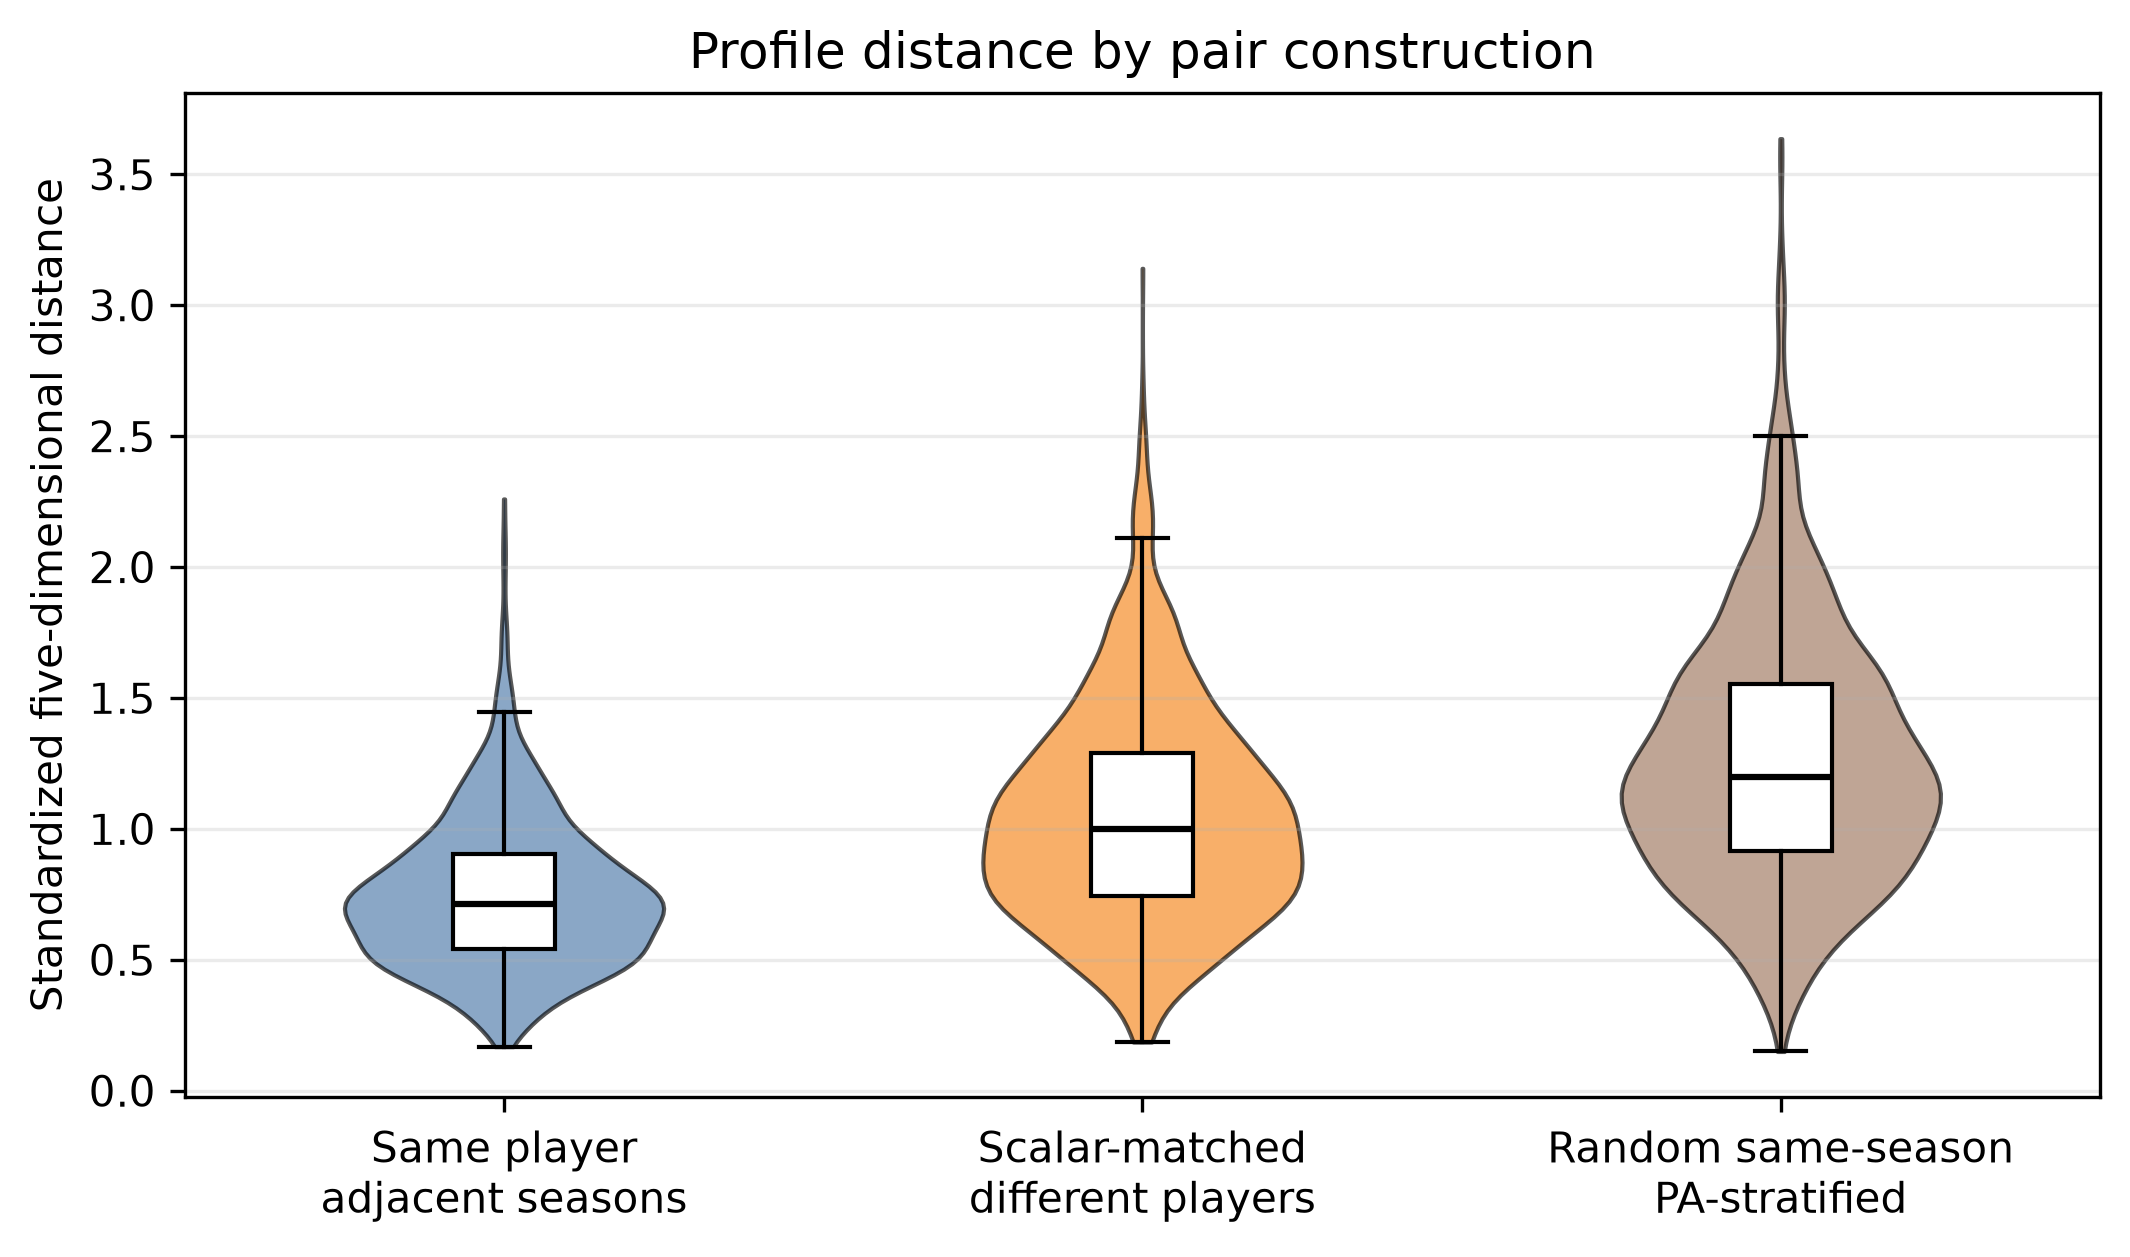
\includegraphics[width=0.92\linewidth]{figures/matched_profile_distances.png}
\caption{Standardized five-dimensional distances for same-player adjacent seasons, different players matched on wRC+ and WAR, and PA-stratified random same-season pairs. Right: a rule-selected scalar-matched example. Scores remain cohort-relative, not scouting grades.}
\label{fig:matched-profile}
\end{figure*}

\subsection{Dimension-Delta Regression and Model Sensitivity}
\label{sec:roi-results}
Table~\ref{tab:cv} reports the $\Delta$Tool regression's $R^2$ under the three cross-validation schemes of Sec.~\ref{sec:roi-method}, for both the five-feature linear model and the ten-feature random forest.

\begin{table*}[t]
\centering
\caption{$R^2$ for contemporaneous dimension-delta associations over 1{,}414 stable-ID transitions. Pooled uses shuffled five-fold \texttt{KFold}; grouped uses player-level \texttt{GroupKFold}; temporal trains on transitions ending by 2023 ($n=701$) and tests on 2024$\to$2025 ($n=358$). The temporal column is not prospective because $\Delta\mathbf{v}$ includes the outcome season.}
\label{tab:cv}
\small
\begin{tabular}{lcccccc}
\toprule
 & \multicolumn{2}{c}{Pooled KFold} & \multicolumn{2}{c}{Player-grouped} & \multicolumn{2}{c}{Temporal holdout} \\
\cmidrule(lr){2-3} \cmidrule(lr){4-5} \cmidrule(lr){6-7}
Target & LR & RF & LR & RF & LR & RF \\
\midrule
$\Delta$wRC+ & 0.707 & 0.678 & 0.708 & 0.680 & 0.701 & 0.634 \\
$\Delta$WAR  & 0.704 & 0.662 & 0.701 & 0.666 & 0.690 & 0.645 \\
$\Delta$OPS  & 0.708 & 0.684 & 0.709 & 0.681 & 0.728 & 0.693 \\
\bottomrule
\end{tabular}
\end{table*}

Player-grouped scores closely track pooled scores across targets and models (Table~\ref{tab:cv}), indicating that the reported fit is not primarily caused by overlapping transitions from the same player. The random forest weakens under temporal separation, while the linear model is comparatively stable. This pattern may reflect time-specific nonlinear structure, but it remains a contemporaneous association because both $\Delta\mathbf{v}$ and the target use the ending season. In the stable-ID linear model, a one-point change in Power is associated with $+3.15$ wRC+, Contact with $+2.17$, and Discipline with $+0.70$, conditional on the other dimension changes; Speed ($-0.13$) and Defense ($+0.04$) are near zero for this offense-only target. Shared underlying statistics make these descriptive partial associations rather than causal exchange rates.

Applying a synthetic $+5$-grade perturbation to each dimension produces player-specific fitted-model responses. For Aaron Judge, the largest response is assigned to Power ($+12.6$ wRC+); for Byron Buxton, it is assigned to Contact ($+14.3$ wRC+). There is no observed ground truth that either dimension is the player's optimal development target, and perturbations may leave the joint data manifold. These are sensitivity examples, not counterfactual outcomes, ROI, or prescriptions.

\begin{figure}[t]
\centering

\includegraphics[width=\linewidth]{figures/roi_coefficients.png}
\caption{Linear-regression coefficients associating concurrent year-over-year dimension changes with changes in value metrics. Coefficients are descriptive associations, not causal exchange rates.}
\label{fig:roi}
\end{figure}

\subsection{Sensitivity Analysis}
Because pentagon area sums adjacent products (Eq.~\ref{eq:area}), it is not permutation-invariant. Population-level correlations vary only within $\pm 0.02$ across orderings, but individual rankings can change substantially as within-player dimension variance increases. Thus, the ``spiky'' profiles for which the full vector is most informative are also those for which radar-chart area is least stable. This finding limits area as a comparison metric and supports using it only as an auxiliary geometric descriptor.

Several planned construction-level checks could not be completed from the archived output: no-/double-shrinkage variants, leave-one-statistic-out encodings, alternative Defense definitions, a constituent raw-statistic predictor, and multi-seed JointVAE stability all require source-level features or model artifacts that are absent. Their absence should be read as unresolved robustness, not as negative evidence. The available results support the usefulness of the released five-dimensional output, but do not identify which upstream design choices are necessary.


\section{Conclusion and Limitations}
\label{sec:conclusion}

We presented Baseball2Vector, a mapping from public season statistics to an interpretable five-dimensional, cohort-relative profile. The strongest evidence is no longer the shared-input area correlation alone. In a fixed 2024$\to$2025 test, the five dimensions carry modest but statistically supported next-season wRC+ signal beyond league-mean and carry-forward baselines; scalar-matched players also remain substantially farther apart in profile space than the same player across adjacent seasons. Together, these findings support Baseball2Vector as a compact descriptive interface with some predictive content. They do not validate it as a scouting scale, show that it is superior to its unavailable raw inputs, or justify causal development recommendations.

\paragraph{Limitations.}
The area correlations remain circular because several inputs contribute directly or indirectly to WAR, wRC+, or OPS, and external construct validity has not yet been established. Min--max scores depend on the cohort; correlated inputs can double-count signals; and Defense is particularly problematic because Def contains Fld plus positional adjustment, so the current average repeats fielding while mixing position, opportunity, and playing time. The prospective test includes only players who returned for at least 100 PA in 2025, creating survivorship and role-selection bias; its bootstrap quantifies test-sample uncertainty for a fixed modeling procedure, not uncertainty over every data-collection and model-selection decision. Matching analyses reuse focal and comparison players, so their intervals apply to the constructed matched sample. Most importantly, the archived file lacks constituent statistics and fitted JointVAE artifacts, preventing raw-input comparison, shrinkage and leave-one-statistic-out checks, alternative Defense constructions, and multi-seed latent stability analysis. Delta regressions use outcome-season changes and therefore remain contemporaneous even under temporal splitting. Synthetic perturbations inherit age, injury, role, and playing-time confounding and may leave the observed data manifold.

\paragraph{Future directions.}
The immediate priority is to preserve a versioned source export with stable IDs and every constituent statistic when FanGraphs access becomes available again. That would permit leakage-controlled raw-statistic baselines, shrinkage and feature-ablation studies, alternative fielding-only and position-adjusted Defense definitions, and multi-seed JointVAE evaluation. External construct validation should use independently verifiable reference data. Prospective tests should include attrition modeling and multiple future seasons, while development claims require subsequently realized changes and explicit adjustment for age, injury, role, position, and playing time. Until then, the appropriate use is profile description, comparison, and hypothesis generation.

%%%%%%%%% REFERENCES
\begin{thebibliography}{99}

\bibitem{mcdaniel2014}
K. McDaniel.
\newblock Scouting explained: The 20--80 scouting scale.
\newblock \emph{FanGraphs Baseball}, 2014. \url{https://blogs.fangraphs.com/scouting-explained-the-20-80-scouting-scale/}.

\bibitem{alcorn2016}
M. A. Alcorn.
\newblock 2vec: Statistic-free talent modeling with neural player embeddings.
\newblock In \emph{MIT Sloan Sports Analytics Conference}, 2016.

\bibitem{heaton2021}
C. Heaton and P. Mitra.
\newblock Learning to describe player form in the MLB.
\newblock \emph{arXiv preprint arXiv:2109.05280}, 2021.

\bibitem{fangraphsSampleSize}
FanGraphs Sabermetrics Library.
\newblock Sample size.
\newblock \url{https://library.fangraphs.com/principles/sample-size/}.

\bibitem{fangraphsDef}
FanGraphs Sabermetrics Library.
\newblock Defensive Runs Above Average (Def).
\newblock \url{https://library.fangraphs.com/defense/def/}.

\bibitem{chadwickRegister}
Chadwick Baseball Bureau.
\newblock Chadwick Register: a repository of baseball player identifiers.
\newblock \url{https://github.com/chadwickbureau/register}.

\bibitem{mikolov2013}
T. Mikolov, K. Chen, G. Corrado, and J. Dean.
\newblock Efficient estimation of word representations in vector space.
\newblock {\em arXiv preprint arXiv:1301.3781}, 2013.

\bibitem{kingma2014}
D. P. Kingma and M. Welling.
\newblock Auto-encoding variational Bayes.
\newblock In {\em ICLR}, 2014.

\end{thebibliography}

\end{document}
